\section{Architecture}\label{sec:architecture}

Web applications developed exploiting \brand{x-project} toolkit are full stack {\em JavaScript}. 

On the server-side they rely on {\em Node.js}, exploiting the power of the {\em Loopback} framework by {\em Strongloop}. As mention above, the aim is to have a development process entirely document-driven, and those documents are the schemas of the models used by the application. These are JSON documents. Each document represents a model and presents the following fields: the \texttt{name} of the model, the set of \texttt{properties}, the list of \texttt{relations} to others models and the list of \texttt{ACL} (Access Control Layer) rules. 

{\em Loopback} generates model’s API from the models schemas, to let CRUD operations on models.

The API can be extended: the developer can add remote functions to models or add hooks to existing APIs to add behaviour before and/or after the API handler (to preprocess the request and/or postprocess the response). 


The resulting API is RESTful, cookie free, signed by authentication token.

By default, applications have a built-in model that represent a user, with
properties \texttt{username}, \texttt{email} and \texttt{password} for login
and the property \texttt{role} used by the ACL module.

A very remarkable feature exposed by {\em Loopback} is that it abstracts from the particular DBMS utilized by the mean of an indirection layer, allowing to choose the preferred one, be it a noSQL or a graph-based one.


On the client-side, developed applications happen to be SPA (single page
application) which exploit a variety of technologies, briefly described below.

\begin{description}
\itemsep1pt\parskip0pt\parsep0pt

\item[Web Components] are a collection of standards which are working their way through the W3C and landing in browsers at the moment. They allow to bundle markup and styles into custom HTML elements. \emph{Custom Elements}\cite{custom-elements}, \emph{HTML Imports}\cite{html-imports}, \emph{HTML Templates}\cite{html-templates}, \emph{Shadow DOM}\cite{shadow-dom}. Since these specifications are currently W3C Working Draft, they aren’t fully supported across all major browsers, so 
As these technologies are implemented in browsers, the polyfills will shrink to gain the benefits of native implementations. \cite{webcomponents-polyfills} 
        
\item[Polymer library] (\url{https://www.polymer-project.org/}) provides a thin layer of API on top of web components (native implementations and their polyfills) and several powerful features, such as custom events and delegation, mixins, accessors and component lifecycle functions, that makes it easier and faster to create Web Components. Similar to \emph{Polymer} are \emph{x-tag} and \emph{Bosonic}. Web repositories \url{http://component.kitchen} and \url{http://customelements.io} already counts thousands of open source user-contributed custom elements.
\end{description}

% \begin{figure}[!htbp]
% \centering
% 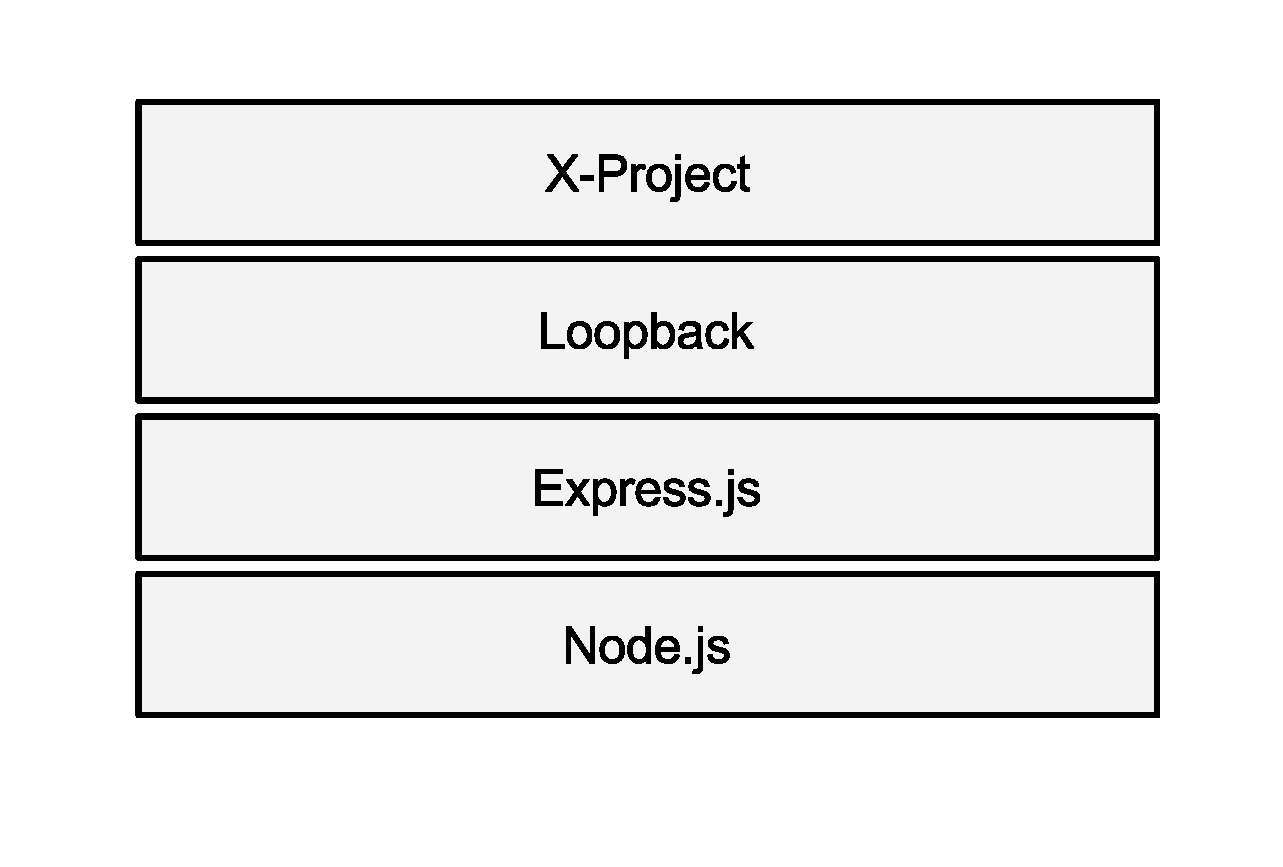
\epsfig{file=images/stack.eps, height=0.2\textwidth}
% \caption{Technology stack}
% \label{fig:tech-stack}
% \end{figure}

% \begin{figure}[!h]
%  \centering
%  \begin{subfigure}[b]{0.53\linewidth}
%  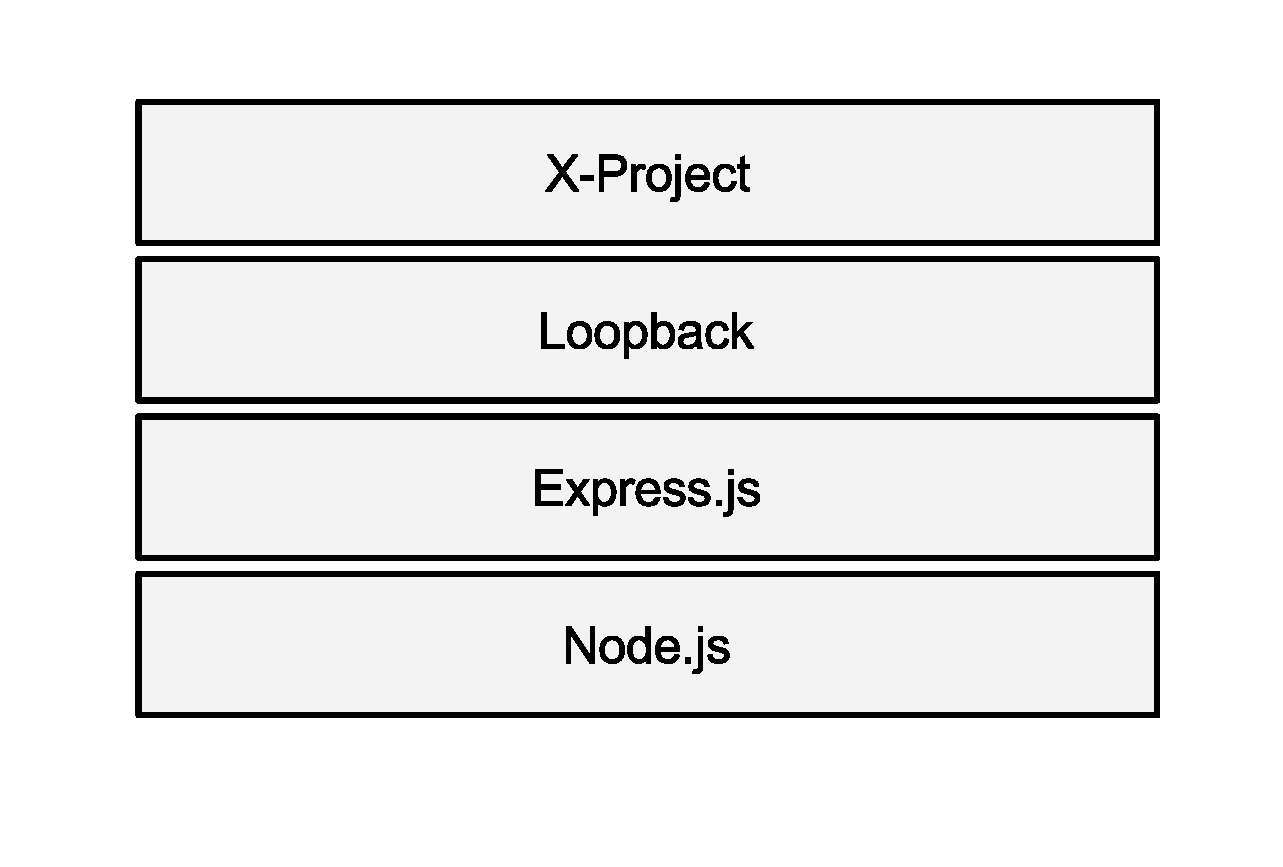
\includegraphics[width=\textwidth]{images/stack.eps} 
%  \caption{Technology stack.}
%  \label{fig:tech-stack}
%  \end{subfigure}
%  ~
%  \begin{subfigure}[b]{0.43\linewidth}
%  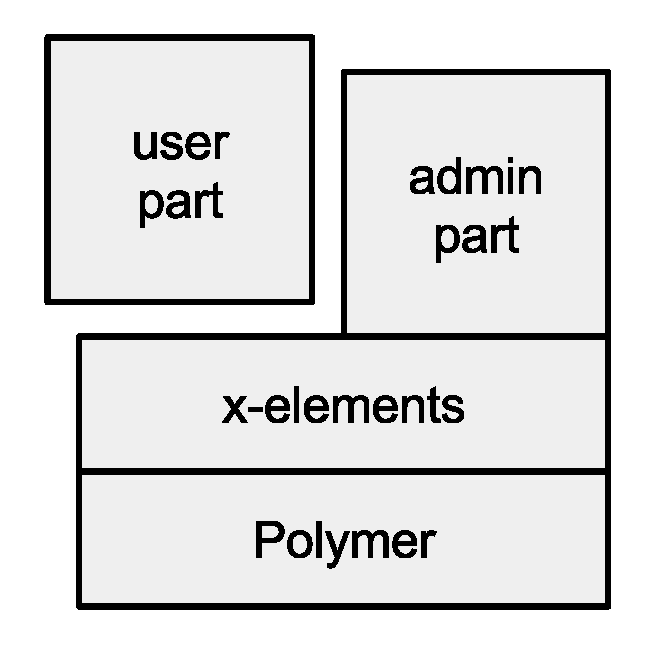
\includegraphics[width=\textwidth]{images/client-arch.eps}
%  \caption{Client-side architecture}
%  \label{fig:client-arch}
%  \end{subfigure}
 
%  % \caption{Office building: 
%  % (a) the schematic plan; 
%  % (b) the simplified 3D model generated for testing on the field 
%  % the indoor mapping project described in this paper.
%  % }
%  % \label{fig:sogei}
% \end{figure}

% \begin{figure}[!htbp]
% \centering
% 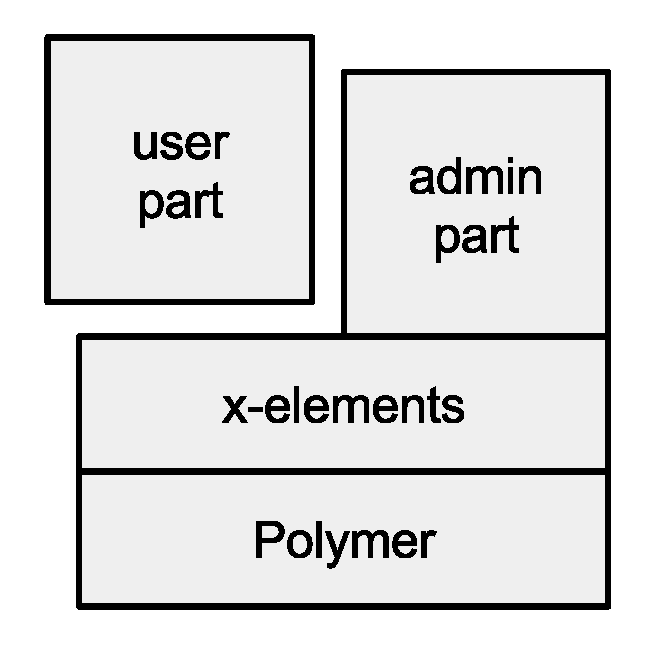
\epsfig{file=images/client-arch.eps, height=0.2\textwidth}
% \caption{Client-side architecture}
% \label{fig:client-arch}
% \end{figure}


% \subsubsection{Third party services}
% \brand{x-project} is designed to be connected to microservices. These tools are accessible extending the Web Application API.

% An essential feature of a CMS is media storage (documents, images and videos) \cite{5552271}. 

% \brand{x-project} provides a remote storage service implemented as a direct upload module to AWS Amazon S3 storage service. The media to upload don’t pass through the server but are sent directly to AWS using a signed request.
% The signature of the request is provided by the module.
% The module has to be configured with the AWS bucket settings: bucket name, public and secret keys. 

% \begin{figure}[!htbp]
% \centering
% 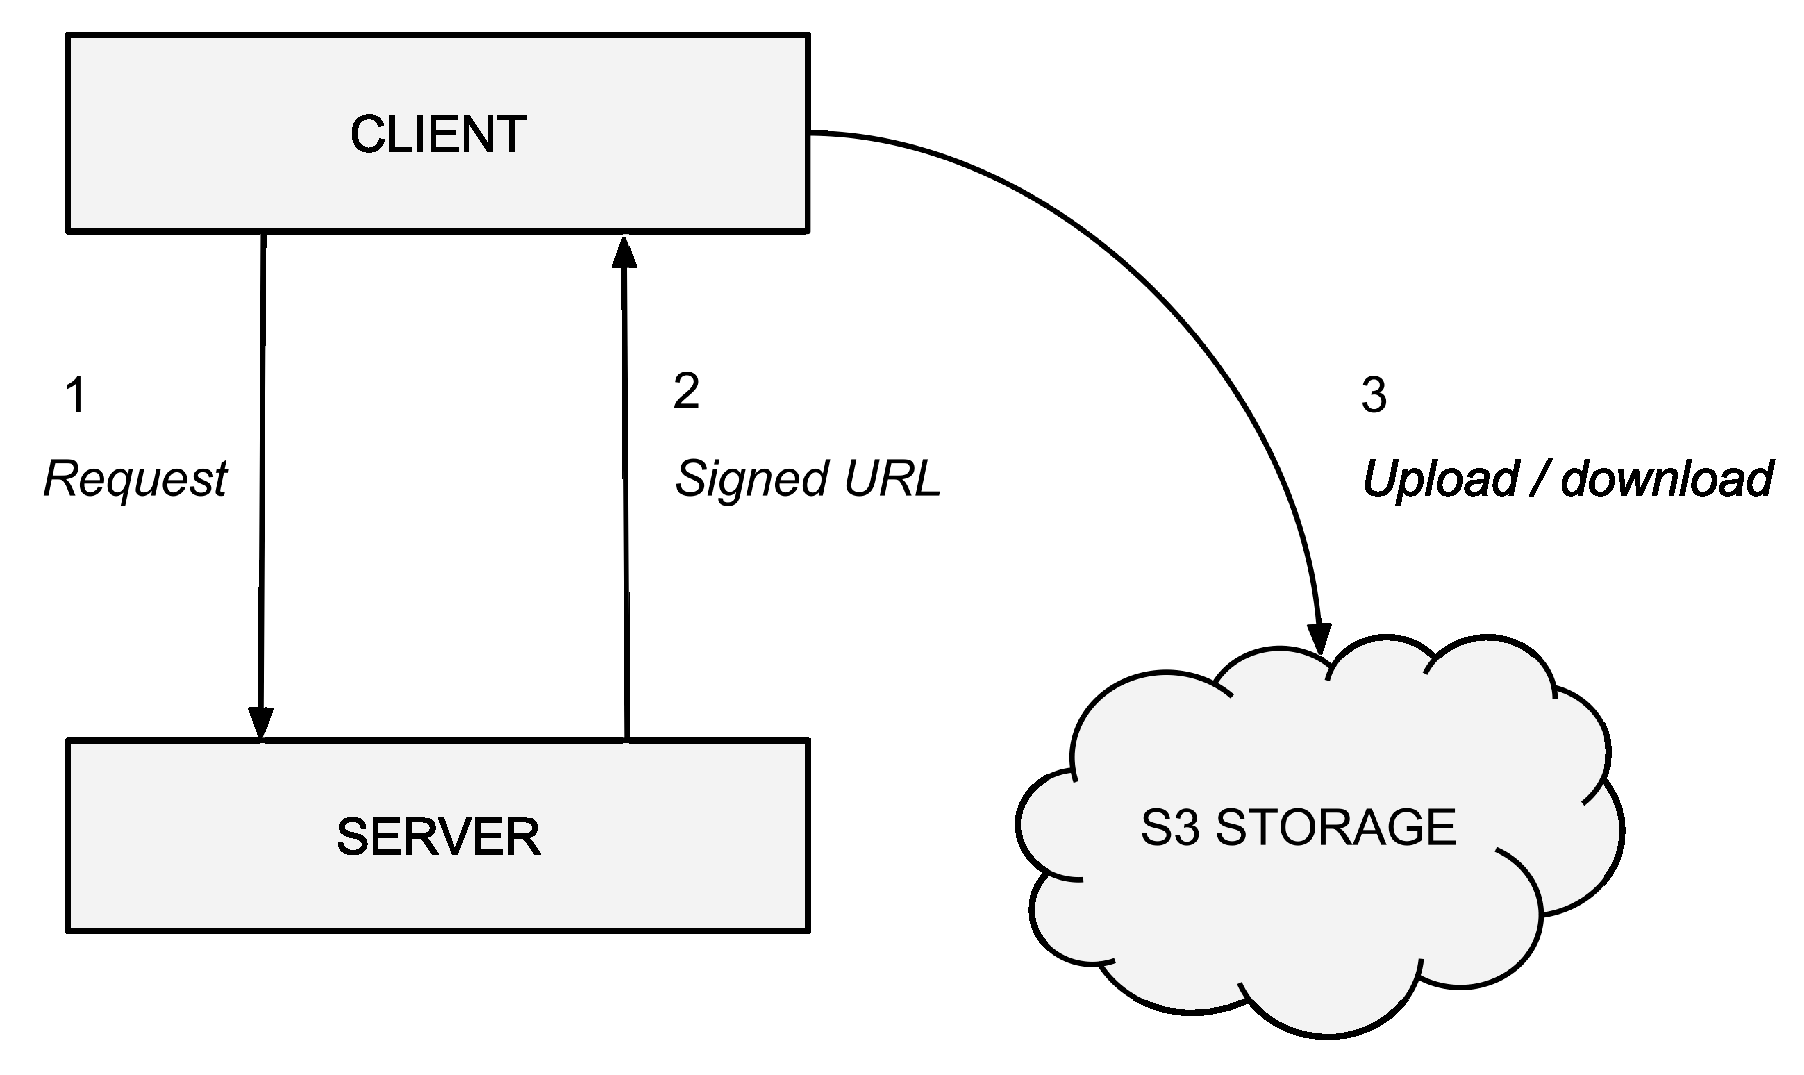
\epsfig{file=images/services.eps, height=0.24\textwidth}
% \caption{Third parties services}
% \label{fig:services}
% \end{figure}
